\documentclass[12pt, answers]{exam}
%\documentclass[12pt]{exam}
\RequirePackage{amssymb, amsfonts, amsmath, latexsym, verbatim, xspace, setspace}
\RequirePackage{tikz, pgflibraryplotmarks}
\usepackage[margin=1in]{geometry}
\usepackage{enumerate, paralist}
\parindent 0ex

\onehalfspacing

\usepackage{amsthm}
\usepackage{epsfig}
\usepackage{times}
\renewcommand{\ttdefault}{cmtt}
\usepackage{graphicx} % for graphics files

% The float package HAS to load before hyperref
\usepackage{float} % for psuedocode formatting

% from Denovo Methods Manual
\usepackage{mathrsfs}
\usepackage[mathcal]{euscript}
\usepackage{color}
\usepackage{array}

\usepackage[pdftex]{hyperref}
\usepackage[parfill]{parskip}
\usepackage{cancel}

\newcommand{\nth}{n\ensuremath{^{\text{th}}} }
\newcommand{\ve}[1]{\ensuremath{\mathbf{#1}}}
\newcommand{\Macro}{\ensuremath{\Sigma}}
\newcommand{\vOmega}{\ensuremath{\hat{\Omega}}}

\begin{document}
\begin{center}
{\bf NE 155, Classes 4-5, S21 \\
TE \\ January 28, 2021}
\end{center}

\setlength{\unitlength}{1in}
\begin{picture}(6,.1) 
\put(0,0) {\line(1,0){6.25}}         
\end{picture}

%-------------------------------------------------------------
\section*{Transport Equation}

Largely from Lewis and Miller Chp.\ 1 \cite{Lewis1993} and Duderstadt and Hamilton Chp.\ 4 \cite{Duderstadt1976}. Note: Duderstadt and Martin \cite{Duderstadt1979} is a very good general reference. It goes through all of this same stuff, but from a slightly more generic point of view (since this applies to \underline{any} collection of neutral particles).

\subsection*{Definitions}
Spatial logistics\\
\begin{minipage}{0.55\textwidth}
\begin{center}
\begin{figure}[H]
    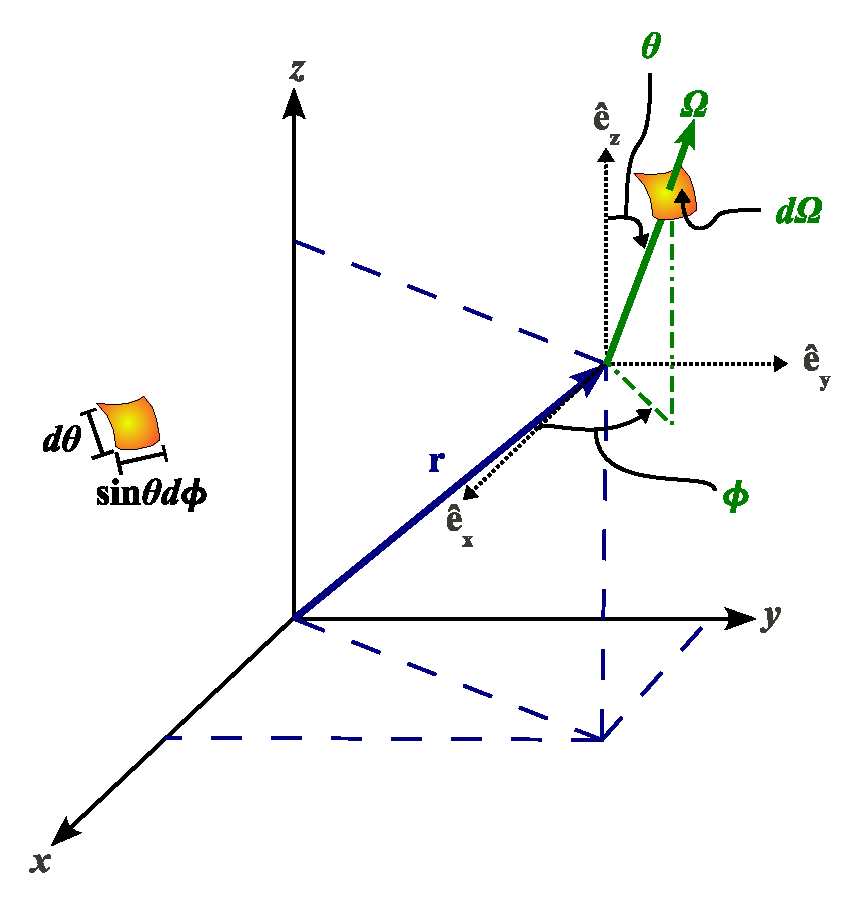
\includegraphics[width = 2.5 in]{../figs/phase_space}
\end{figure}
\end{center}
\end{minipage} \hfill
%
\begin{minipage}{0.45\textwidth}
\begin{figure}[H]
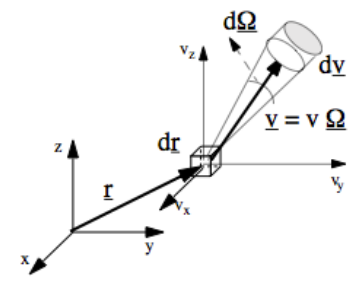
\includegraphics[height=1.5in]{../figs/differential-element}
\end{figure}
\end{minipage}
%
\begin{itemize}
\item $d\vec{r} = d^3r$ = ordinary volume = $r^2 \sin(\theta) d\theta d\varphi dr$
%
\item $v$ = speed (scaler)
\item $\vec{v}$ = velocity (vector)
\ifprintanswers
\item $d\vec{v} = d^3v$ = velocity volume = $v^2 \sin(\theta')d\theta' d\varphi' dr$
\else
 \item \vspace*{2em}
\fi
\item $v = \sqrt{(2E)/m}$ where $m$ is the rest mass of the particle. Thus, we can relate energy and speed.

\item $\vOmega$: unit directional vector in velocity space, $\vec{v} = v\vOmega$
\item $d\vOmega = \sin(\theta')d\theta' d\varphi' =  d^2\Omega$
%\item thus $d\vec{v} = v^2 dv d\vOmega$
\end{itemize}

These are the possible reactions we're generally going to worry about:

\hspace*{1em}total (t): all interactions. We can break total into:
\begin{itemize}
\item scattering (s): a neutron interacts with an atom and bounces off either elastically or inelastically.
\item absorption (a): a neutron is absorbed by a nucleus. If this happens it might
\ifprintanswers
\item fission (f): cause the nucleus to split into two pieces, releasing more neutrons.
\else
 \item \vspace*{2em}
\fi
\end{itemize}

Physics terms we will use:
\begin{enumerate}
\item \textbf{microscopic x-sec} ($\sigma$, [$cm^2$]): measure of the probability that an incident neutron will collide with a specific nucleus; $\sigma_j$ indicates a specific reaction, e.g.\ $j=f$ is fission.

\item \textbf{macroscopic x-sec} ($\Sigma$ [$cm^{-1}$]): measure of the probability per unit path length that an incident neutron will collide with a target
\[\Sigma_j = \sigma_j N\:,\]
where N is the atomic density of the target.

\item \textbf{double-differential scattering x-sec} ($\sigma_s(E, \vOmega \rightarrow E', \vOmega')dE' d\vOmega'$): measure of the probability that a neutron of energy $E$ and moving in direction $\vOmega$ scatters off of a specific nucleus into energy range $[E', E' + dE']$ and direction range $[\vOmega', \vOmega' + d\vOmega']$.

\item \textbf{fission yield} ($\nu(E)$): average \# of neutrons released by a fission induced by a neutron of energy E.

\ifprintanswers
\item \textbf{fission spectrum} ($\chi(E)dE$): average \# of neutrons produced from fission that are born with energy in $[E, E + dE]$. This is normalized such that
\[\int_0^{\infty} \chi(E)dE =1\:.\]
\else
 \item \vspace*{2em}
\fi

\item \textbf{particle angular density} ($n(\vec{r}, E, \vOmega, t)d\vec{r} d\vOmega dE$): expected number of particles in volume element $d^3r$ at $\vec{r}$ whose energies are in $[E, E + dE]$ and direction of motion is in $[\vOmega, \vOmega + d\vOmega]$ at time $t$.

Note:
\begin{align*}
n(\vec{r}, E, \vOmega, t) &= \frac{1}{mv}n(\vec{r}, v, \vOmega, t) \\
n(\vec{r}, v, \vOmega, t) &= v^2 n(\vec{r}, \vec{v}, t) \\
n(\vec{r}, \vec{v}, t) &= \frac{m}{v}n(\vec{r}, E, \vOmega, t)
\end{align*}

\item \textbf{particle density}: ($N(\vec{r},E,t)d^3r dE$): expected number of particles in $d^3r$ at $\vec{r}$ whose energies are in $[E, E + dE]$ at time $t$.
\[N(\vec{r},E,t)d^3r dE = \int_{4\pi} d\vOmega\: n(\vec{r}, E, \vOmega, t)d^3r dE \]

\ifprintanswers
\item \textbf{angular flux}: $\psi(\vec{r}, E, \vOmega, t) \equiv v n(\vec{r}, E, \vOmega, t)$.
\else
 \item 
\fi

\item \textbf{scalar flux}: $\phi(\vec{r},E,t) \equiv v N(\vec{r},E,t)$.
%
\[= \int_{4\pi} d\vOmega\: \psi(\vec{r}, E, \vOmega, t) \]

\item \textbf{interaction rate density}: expected number of $j$ reactions per volume per energy at time $t$.
%
\[\int_{4\pi} d\vOmega \:\Sigma_j v n(\vec{r}, E, \vOmega, t) = \Sigma_j \phi(\vec{r},E,t)\]

\item \textbf{angular current density} or partial current: $\vec{j}(\vec{r}, E, \vOmega, t) = \vec{v} n(\vec{r}, E, \vOmega, t)$; 

$\vec{j}(\vec{r}, E, \vOmega, t) \cdot \hat{e}\: dA\: dE\: d\vOmega$ is the expected number of particles crossing $dA$ along unit direction $\hat{e}$ with energy in $[E, E + dE]$ and direction in $[\vOmega, \vOmega + d\vOmega]$ at time $t$.

\item \textbf{net current}: $\vec{J}(\vec{r}, E, t) $ is the net \# of particles crossing a unit area per second along a direction normal to that area with energies in $[E, E + dE]$ at time $t$.
\[\vec{J}(\vec{r}, E, t) = \int_{4\pi} d\vOmega\: \vOmega \psi(\vec{r}, E, \vOmega, t)\]

\end{enumerate}

%-----------------------------------------
\subsection*{Assumptions}
\begin{enumerate}
\item Particles are point objects ($\lambda = h/(mv))$ is small compared to the atomic diameter): its state is fully described by its location, velocity vector, and a given time. This ignores rotation and quantum effects.

\ifprintanswers
\item Neutral particles travel in straight lines between collisions.

\item Particle-particle collisions are negligible (makes TE linear).

\item Material properties are isotropic (generally valid unless velocities are very low).

\item Material composition is time-independent (generally valid over short time scales).

\item Quantities are expected values: fluctuations about the mean for very low densities are not accounted for.
\else
 \item \vspace*{2em}
  \item \vspace*{2em} 
   \item  \vspace*{2em}
    \item \vspace*{2em}
     \item \vspace*{2em}
\fi
\end{enumerate}


%-----------------------------------------
\section*{Derivation}
The TE is a \underline{detailed} balance of the particle population over phase space that is as close to exact as possible. 

DRAW a Differential volume picture.

Consider a volume $V$ with surface $S$. For each point $\vec{r} \in S$, let $\hat{e}_S$ be the outward normal vector.

For a given $\vOmega$, define $S^+$ as that part of $S$ for which $\hat{e}_S \cdot \vOmega > 0$ (outgoing particles) and $S^-$ as that part of $S$ for which $\hat{e}_S \cdot \vOmega < 0$ (incoming particles).

Then, for this volume $V$ for a fixed $E$ and $\vOmega$, the general rate equation can be written for particles satisfying $\vec{r} \in V$, energies in $[E, E+dE]$ and direction $[\vOmega, \vOmega + d\vOmega]$ as:

\ifprintanswers
\hspace*{3 em} \boxed{\text{Rate of change of the particle (neutron) population 
 = rate of production - rate of loss}}
\else
 \vspace*{2em}
\fi

%--------------
\subsection*{Rate of Change}
Recall the definition of $n$: expected number of particles in volume element $d^3r$ at $\vec{r}$ whose energies are in $[E, E + dE]$ and direction of motion is in $[\vOmega, \vOmega + d\vOmega]$ at time $t$.

To get the rate of change of particles within the volume, we need to integrate over volume and take the derivative with respect to time:

\ifprintanswers
\[\boxed{\Bigl[ \int_V \frac{\partial}{\partial t} n(\vec{r}, E, \vOmega, t) d\vec{r} \Bigr] dE d\vOmega }\]
\else
 \vspace*{3em}
\fi


%--------------
\subsection*{Production Mechanisms}
How can we produce neutrons in volume element $d^3r$ at $\vec{r}$ whose energies are in $[E, E + dE]$ and direction of motion is in $[\vOmega, \vOmega + d\vOmega]$ at time $t$?
%
\begin{enumerate}
\ifprintanswers
\item Inscattering (from some other energy and/or angle into our energy and angle),
\else
 \item \vspace*{2em}
\fi
\item Fission neutrons, or
\item Fixed/interior sources.
\end{enumerate}

1) Scattering into $[E, E + dE]$ and $[\vOmega, \vOmega + d\vOmega]$

This is the definition of the double differential scattering cross section:
\[\boxed{\Bigl[\int_V d^3r \int_{4\pi} d\vOmega' \int_0^{\infty} dE' \: \Sigma_s(E', \vOmega' \rightarrow E, \vOmega) v' n(\vec{r}, E', \vOmega', t) \Bigr] dE d\vOmega}\]

2) Expected rate of neutron production by fission

Note: fission neutrons are isotropic, thus they are produced at $\frac{1}{4\pi}$ per steradian. This means the fraction within $[\vOmega, \vOmega + d\vOmega]$ is $\frac{d\vOmega}{4\pi}$ (fyi: including this normalization differs among textbooks and research papers).

Also, recall that $\chi(E)dE$ is the fraction of neutrons born into $[E, E + dE]$. Thus
%
\ifprintanswers
\[\boxed{\frac{\chi(E)}{4\pi}\Bigl[\int_V d^3r \int_{4\pi} d\vOmega' \int_0^{\infty} dE' \: \nu(E') \Sigma_f(E') v' n(\vec{r}, E', \vOmega', t) \Bigr] dE d\vOmega}\]
\else
\\ \\ \vspace*{2em}
\fi

3) Production from a fixed source

Sources are fully specified by a function reminiscent of the $n$ definition: $s(\vec{r}, E, \vOmega, t)$ s.t.\ \\$s(\vec{r}, E, \vOmega, t)d^3rdEd\vOmega \equiv$ the expected number of particles that are produced at time $t$ inside volume $d^3r$ at $\vec{r}$ with energy $[E, E + dE]$ and direction $[\vOmega, \vOmega + d\vOmega]$.

Rate of production of such particles in $V$ is
\[\boxed{\Bigl[\int_V d^3r \:s(\vec{r}, E, \vOmega, t) \Bigr] dE d\vOmega }\]

%--------------
\subsection*{Loss Mechanisms}
How can we lose neutrons from volume element $d^3r$ at $\vec{r}$ whose energies are in $[E, E + dE]$ and direction of motion is in $[\vOmega, \vOmega + d\vOmega]$ at time $t$?
%
\begin{enumerate}
\setcounter{enumi}{3}
\item Neutrons can collide and exit the phase space (any collision will change its state) or
\item Neutrons can stream into other locations and/or directions of motion (leakage).
\end{enumerate}

4) Total interaction: any collision can lead to (a) absorption or (b) a change in $E$ or $\vOmega$ or both.

\ifprintanswers
\[\boxed{\Bigl[\int_V d^3r \Sigma_t(E) v n(\vec{r}, E, \vOmega, t) \Bigr] dE d\vOmega }\]
\else
\vspace*{3em}
\fi

5) Net leakage out of phase space

\begin{figure}[h!]
\begin{center}
%\includegraphics[height=1in]{UnitXsecArea}
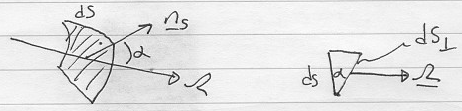
\includegraphics[height=1in]{../figs/DifferentialArea}
\end{center}
\end{figure}

Use the definition of $\vec{j} \rightarrow$ the expected number of particles crossing $dS$ along $\hat{e}_S$ with energy $[E, E + dE]$ and direction $[\vOmega, \vOmega + d\vOmega]$ at time $t$  
%
\[= \vec{j}(\vec{r}_s, E, \vOmega, t) \cdot d\vec{S} dE d\vOmega\:,\]
%
where $\vec{r}_s$ is a point on the surface and $d\vec{S} = \hat{e}_S dS$.

Thus, the total leakage out of $V$ is
\[\Bigl[\int_S \vec{j}(\vec{r}_s, E, \vOmega, t) \cdot d\vec{S} \Bigr] dE d\vOmega\:. \]

We can use divergence theorem to rewrite this w.r.t.\ $V$ (rather than $S$):
\[\int_S \hat{e}_S \cdot \vec{F} (\vec{r}) dS = \int_V \nabla \cdot \vec{F} (\vec{r}) dV\]
%where
%\[\nabla = \vec{i}\frac{d}{dx} + \vec{j}\frac{d}{dy} + \vec{k}\frac{d}{dz}\]
%is the gradient operator.

This gives
\ifprintanswers
\[\Bigl[\int_V d^3r \: \nabla \cdot \bigl( \underbrace{\vec{j}(\vec{r}_s, E, \vOmega, t)}_{=\vec{v}n = v \vOmega n} \bigr) \Bigr] dE d\vOmega \]
\else
\\ \vspace*{3em}\\
\fi
%
And we can use this identity:
\begin{align}
%
\vOmega \cdot (\nabla f) &= \nabla \cdot \vOmega f \text{ because }\vOmega\text{ is not a function.} \nonumber\\
\nabla \cdot \vOmega f &= f(\underbrace{\nabla \cdot \vOmega}_{0}) + \vOmega \cdot (\nabla f) \nonumber
\end{align}
%
\ifprintanswers
\[\therefore \:\: \boxed{\Bigl[\int_V d^3r \: \vOmega \cdot \nabla \bigl(v n(\vec{r}_s, E, \vOmega, t) \bigr) \Bigr] dE d\vOmega }\]
\else
\vspace*{3em}
\fi

Note: $\vOmega \cdot \nabla$ represents the derivative along the direction of motion.

%--------------
\subsection*{All Together Now}
The balance of neutrons: rate of change - production + loss = 0.

Suppressing dependencies to save space for the moment
%
\begin{align}
\int_V d^3r \Bigl[\frac{\partial n}{\partial t} &- 
\int_{4\pi} d\vOmega' \int_0^{\infty} dE' \:\Sigma_s(E', \vOmega' \rightarrow E, \vOmega) v' n' \nonumber\\&-
\frac{\chi(E)}{4\pi} \int_{4\pi} d\vOmega' \int_0^{\infty} dE' \:\nu(E') \Sigma_f(E') v' n' -
s +
\Sigma_t v n + 
\vOmega \cdot \nabla v n \Bigr] = 0 \nonumber
\end{align}

We note that since the volume was arbitrarily chosen, the integral will only vanish if the integrand is zero 
\[\int_{\text{any }V} d^3r f(\vec{r}) = 0 \rightarrow f(\vec{r}) = 0 \:.\]

Now we have a balance relation that we can rearrange, substituting $\psi(\vec{r}, E, \vOmega, t) = vn(\vec{r}, E, \vOmega, t)$, to get what we usually call the Boltzmann Equation for neutron transport
%
\begin{align}
\frac{1}{v}\frac{\partial \psi(\vec{r}, E, \vOmega, t)}{\partial t} &+ 
\vOmega \cdot \nabla \psi(\vec{r}, E, \vOmega, t) +
\Sigma_t \psi(\vec{r}, E, \vOmega, t) = \nonumber\\
%
& \int_{4\pi} d\vOmega' \int_0^{\infty} dE' \Sigma_s(E', \vOmega' \rightarrow E, \vOmega) \psi(\vec{r}, E', \vOmega', t)  +\nonumber\\
%
& \frac{\chi(E)}{4\pi} \int_0^{\infty} dE' \nu(E') \Sigma_f(E') \int_{4\pi} d\vOmega' \psi(\vec{r}, E', \vOmega', t) +
s(\vec{r}, E, \vOmega, t) \nonumber
\end{align}

%--------------
\subsection*{Initial and Boundary Conditions}
\begin{enumerate}
\item \underline{Initial Condition}: we start with some initial ``known" state:
\ifprintanswers
\[\psi(\vec{r}, E, \vOmega, 0) = \psi_0(\vec{r}, E, \vOmega)\]
\else
\\ \vspace*{3em}\\
\fi
for the problem domain. Note, the initial flux can be a functional expression.

\item \underline{Interface Condition}: the angular flux must be continuous along $\vOmega$ at all points, including material interfaces.

\begin{minipage}{0.45\textwidth}
\begin{figure}[H]
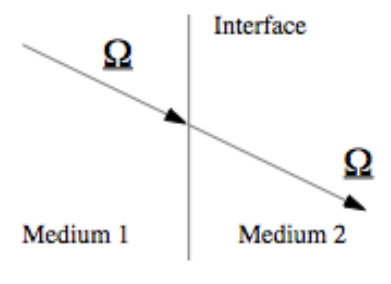
\includegraphics[height=2in]{../figs/interface}
%\caption{\label{fig:interfaceCondition} Interface Condition}
\end{figure}
\end{minipage} \hfill
\begin{minipage}{0.45\textwidth}
$\psi_1(\vec{r}_S, E, \vOmega, t) = \psi_2(\vec{r}_S, E, \vOmega, t)$

\vspace*{1 em}
$\forall E$ and $\vOmega$.
\end{minipage}

\item \underline{Fixed Condition}: you can specify incoming flux

\begin{minipage}{0.45\textwidth}
\begin{figure}[H]
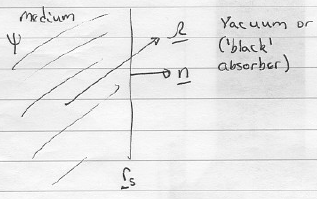
\includegraphics[height=1.75in]{../figs/FreeSurfaceCondition}
%\caption{\label{fig:FixedCondition} Fixed Condition}
\end{figure}
\end{minipage} \hfill
\begin{minipage}{0.45\textwidth}
$\psi(\vec{r}_S, E, \vOmega, t) = \psi_{IN}(\vec{r}_S, E, \vOmega, t)$ for \\$\vec{e} \cdot \vOmega < 0$: specifying incoming neutrons. Note, the incoming flux can be a functional expression; it can also be zero.

This is equivalent to specifying the incoming partial current, $$\vec{j}^-(\vec{r}_S, E, t) = \int_{\vec{e} \cdot \vOmega < 0} d\vOmega \:(\vec{e} \cdot \vOmega) \psi(\vec{r}_S, E, \vOmega, t)\:.$$
\end{minipage}

\item \underline{Reflective Condition}: there is mirror symmetry at some surface:\\
\begin{minipage}{0.75\textwidth}
\begin{figure}[H]
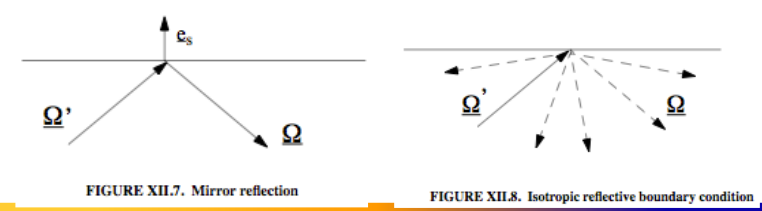
\includegraphics[height=1.25in]{../figs/reflecting-bc}
\end{figure}
\end{minipage} \hfill
\begin{minipage}{0.25\textwidth}
\ifprintanswers
\[\psi(\vOmega_{IN}) = \psi(\vOmega_{OUT})\:.\]
\else
\\ \\ \vspace*{2em}
\fi
\end{minipage}

\item \underline{Periodic Condition}: you know there is a repetition in the system\\
\begin{minipage}{0.5\textwidth}
\begin{figure}[H]
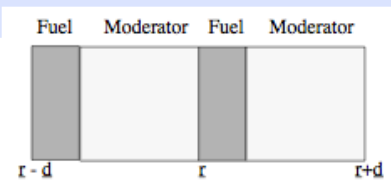
\includegraphics[height=1.25in]{../figs/periodic-bc}
\end{figure}
\end{minipage}
\begin{minipage}{0.5\textwidth}
\[\psi(\vec{r}_S, E, \vOmega, t) = \psi(\vec{r}_S \pm \vec{p}, E, \vOmega, t)\:.\]
\end{minipage}

\item \underline{Finiteness Condition}: to by physically valid we need to meet the condition \\$0 < \psi(\vec{r}, E, \vOmega, t) < \infty$, with the possible exception of point sources,

\item which we handle with the \underline{Source Condition}: localized sources are introduced as mathematical singularities at the location of the source.

For a source $s(\vec{r}_0, E, \vOmega, t)$:
\\
\begin{minipage}{0.25\textwidth}
\begin{figure}[H]
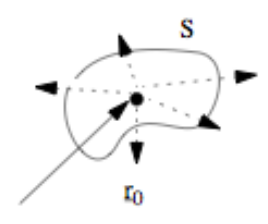
\includegraphics[height=1.25in]{../figs/source}
\end{figure}
\end{minipage}
\begin{minipage}{0.75\textwidth}
\ifprintanswers
\begin{align*}
&\lim_{\vec{r} \rightarrow \vec{r}_0} \int_S dS\: \vec{e} \cdot \vOmega \psi(\vec{r}, E, \vOmega, t) = s(\vec{r}_0, E, \vOmega, t)\:, \\
&s(\vec{r}, E, \vOmega, t) = s(\vec{r}_0, E, \vOmega, t)\delta(\vec{r} - \vec{r}_0)\:.
\end{align*}
\else
\\ \\ \vspace*{2em}
\fi
\end{minipage}
\end{enumerate}


%---------------------------------------------
%---------------------------------------------
\section*{Simplified Forms}

\subsection*{One Speed}
Assume all particles are at the same speed, so we no longer need energy dependence.

%We assume all particles have the same speed, $\vec{v} = v_0 \cdot \vOmega$. Thus
%%
%\begin{align}
%n(\vec{r}, v, \vOmega, t) &= n(\vec{r}, \vOmega, t) \delta(v - v_0) \\
%\Sigma_s(\underbrace{E' \rightarrow E, \vOmega' \cdot \vOmega}_{\text{another way to write this}}) &= \Sigma_s(E,\vOmega' \cdot \vOmega)\delta(E' - E)
%\end{align}
%
% remove E integration and E dependence

\begin{align*}
\frac{1}{v}\frac{\partial \psi(\vec{r}, \vOmega, t)}{\partial t} &+ 
\vOmega \cdot \nabla \psi(\vec{r}, \vOmega, t) +
\Sigma_t \psi(\vec{r}, \vOmega, t) = \nonumber\\
%
& \int_{4\pi} d\vOmega' \Sigma_s(\vOmega' \rightarrow \vOmega) \psi(\vec{r}, \vOmega', t)  
+ \frac{\nu \Sigma_f}{4\pi} \int_{4\pi} d\vOmega' \psi(\vec{r},  \vOmega', t) 
+ s(\vec{r}, \vOmega, t) 
%Q(\vec{r}, \vOmega, t)
\end{align*}
%
%Where:
%\begin{align}
%Q(\vec{r}, \vOmega, t) &= \frac{1}{4\pi} \nu \Sigma_f \int_{4\pi} d\vOmega' \psi(\vec{r},  \vOmega, t) + S(\vec{r}, \vOmega, t) \\
%&= \frac{1}{4\pi} \bigl( \nu \Sigma_f \phi(\vec{r}, t) + s(\vec{r}, t) \bigr)
%\end{align}


%---------------------------------------------
\subsection*{One Speed, One Dimensional}

We'd like to simplify even farther by only worrying about one dimension, so we'll get rid of $y$ and $z$.

\begin{minipage}{0.5\textwidth}
$\vec{r} = (x, y, z)$
$d\vOmega = \sin(\theta) d\theta	d\varphi = d\mu d\varphi$

Note $\mu = \cos(\theta)$ so $d\mu = \sin(\theta)$

$\Omega_x = \cos(\theta) = \mu$

(in the image mentally swap $y$ and $z$ to get the notation we are using)
\end{minipage}
%
\begin{minipage}{0.5\textwidth}
\begin{figure}[H]
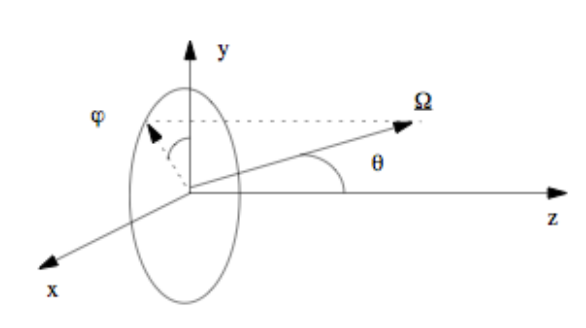
\includegraphics[height=1.5in]{../figs/azimuthal}
%\caption{\label{fig:FixedCondition} Fixed Condition}
\end{figure}
\end{minipage} \hfill
%
\begin{align*}
\frac{1}{v}\frac{\partial \psi(x, \vOmega, t)}{\partial t} &+ 
\bigl(\Omega_x \frac{\partial}{\partial x} + \cancel{\Omega_y \frac{\partial}{\partial y}} + \cancel{\Omega_z \frac{\partial}{\partial z}} \bigr)\psi(x, \vOmega, t) +
\Sigma_t \psi(x, \vOmega, t) = \nonumber\\
%
& \int_{4\pi} d\vOmega' \Sigma_s(\vOmega' \rightarrow \vOmega) \psi(x, \vOmega', t)  + 
\frac{\nu \Sigma_f}{4\pi} \int_{4\pi} d\vOmega' \psi(x,  \vOmega', t) + s(x, \vOmega, t)%+ Q(x, \vOmega, t) \nonumber
\end{align*}

Using this idea we can write things more cleanly:
%
% switch to just \mu
\begin{align*}
\frac{1}{v_0}\frac{\partial \psi(x, \vOmega, t)}{\partial t} &+ 
\mu \frac{\partial}{\partial x}\psi(x, \vOmega, t) +
\Sigma_t \psi(x, \vOmega, t) = \nonumber\\
%
& \int_0^{2\pi} d\phi \int_{4\pi} d\vOmega' \Sigma_s(\vOmega' \cdot \vOmega) \frac{\psi(x, \mu', t)}{2\pi}  + 
\frac{1}{4\pi} \nu \Sigma_f \int_0^{2\pi} d\phi \psi(x, \mu, t) + s(x, \mu, t)% 2\pi Q(x, \mu, t)
\end{align*}

If \textbf{scattering is also isotropic}:
\[\Sigma_s(\vOmega' \cdot \vOmega) = \frac{\Sigma_s}{4\pi} \]

And we get the 1-group, 1-D, isotropic neutron TE:
%
% scattering is now iso, add in sources
\begin{align*}
\frac{1}{v_0}\frac{\partial \psi(x, \mu, t)}{\partial t} &+ 
\mu \frac{\partial}{\partial x}\psi(x, \mu, t) +
\Sigma_t \psi(x, \mu, t) = \nonumber\\
%
& \frac{1}{2} \Sigma_s \int_{-1}^{1} d\mu' \psi(x, \mu', t)  
+  \frac{1}{2} \bigl( \nu \Sigma_f \phi(x, t) + S(x, t) \bigr)
\end{align*}

%---------------------------------------------
\subsection*{Steady State}
If we get rid of time dependence.
%
\begin{equation}
\mu \frac{\partial}{\partial x}\psi(x, \mu) +
\Sigma_t \psi(x, \mu) = \frac{1}{2} \Sigma_s \int_{-1}^{1} d\mu' \psi(x, \mu')  
+  \frac{1}{2} \bigl( \nu \Sigma_f \phi(x) + S(x) \bigr) \nonumber
\end{equation}


And very finally - we can have the unrealistic case of \textbf{purely absorbing media}:
%
\begin{equation}
\mu \frac{\partial}{\partial x}\psi(x, \mu) +
\Sigma_a \psi(x, \mu) = \frac{1}{2} \bigl( \nu \Sigma_f \phi(x) + S(x) \bigr) \nonumber
\end{equation}


%--------------------------------------------
%--------------------------------------------
%--------------------------------------------


%--------------------------------------------------------------------
\bibliographystyle{plain}
\bibliography{../05-de/te-de} 

\end{document}
